\item A ball of mass \( m \) moving with velocity \( v_0 \) experiences a head-on elastic collision with one of the spheres of a stationary rigid dumbbell as shown in Fig. 1.50. The mass of each sphere equals \( m/2 \), and the distance between them is \( l \). Disregarding the size of the spheres, find the proper angular momentum \( \tilde{M} \) of the dumbbell after the collision, i.e. the angular momentum in the reference frame moving translationally and fixed to the dumbbell’s centre of inertia.
    \begin{center}
        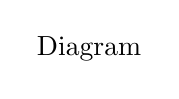
\begin{tikzpicture}
            \node at (0, 0) {Diagram};
        \end{tikzpicture}
    \end{center}\begin{solution}
    \begin{center}
        \begin{tikzpicture}
            \pic at (0, 0) {frame=3cm};
        \end{tikzpicture}
    \end{center}
    
    \begin{align*}
        \intertext{Taking striking ball as particle 1 and upper ball or the dumbbell as particle 2 the velocity acquired by particle 2 on collision, from the formula}
        \vec{v}_{i}^{'} &= 2 \vec{v}_{C} - \vec{v}_{i} \tag{see solution of problem 1.168}\\
        \vec{v}_{2}^{'} &= 2 \left( \dfrac{m v_{0}}{m + m/2} \right) - 0 = \dfrac{4}{3} v_{0}
          \intertext{To find the proper angular momentum of the dumbbell, let
          us denote upper ball of the dumbbell as particle 1 and
          lower ball as particle 2. Then proper angular momentum vector is}
          \vec{\mathcal{M}} &= \vec{r}_{1C} \times m_{1} \vec{v}_{1C} + \vec{r}_{2C} \times m_{2} \vec{v}_{2C} = \vec{r}_{1C} \times \vec{\mathcal{P}}_{1} + \vec{r}_{2C} \times \vec{\mathcal{P}}_{2} 
          \intertext{In C.M. frame net linear momentum of any system is zero, so, $\vec{\mathcal{P}}_{1} = -\vec{\mathcal{P}}_{2}$. So,}
          \vec{\mathcal{M}} &= (\vec{r}_{1C} - \vec{r}_{2C}) \times \vec{\mathcal{P}}_{1}  = \vec{r}_{12} \times \vec{\mathcal{P}}_{1}
          \intertext{We have}
           \vec{\mathcal{P}}_{1} &= \mu \left( \vec{v}_{1} - \vec{v}_{2} \right)  \tag{see solution of problem 1.147}\\
          &= \dfrac{m}{4} \left( \dfrac{4 v_{0}}{3} i - 0 \right)  = \dfrac{m v_{0}}{3} i
          \intertext{Hence,}
          \vec{\mathcal{M}} &= \left[ \vec{r_{12}} \times \vec{\mathcal{P}}_{1}  \right] = \left[ j \times  \dfrac{m v_{0}}{3} i \right] = \dfrac{mv_{0} l}{3} (-k)
          \intertext{Hence,}\\
         \vec{\mathcal{M}} &=  \dfrac{mv_{0} l}{3}
    \end{align*}
\end{solution}